\documentclass[8pt,a4paper]{article}

\usepackage{geometry}
\usepackage{graphicx}
\usepackage{ragged2e}
\usepackage{multicol}
\usepackage{caption}

\usepackage{listings}
\usepackage{xcolor}

\lstset{
  basicstyle=\ttfamily\normalfont\scriptsize,
  breakatwhitespace=true,         
  escapeinside={\%*}{*)},
  breakautoindent=true,
  breaklines=true,                 
  captionpos=b,                    
  keepspaces=false,                 
  showspaces=false,                
  showstringspaces=false,
  showtabs=false,                  
  frame=single,
  numbers=none,
  stepnumber=1,% the step between two line-numbers. If it's 1 each line will be numbered
  tabsize=2
}

% Bash
\lstdefinelanguage{Bash}{
  morekeywords={
    if,then,else,elif,fi,for,while,do,done,case,esac,export
  },
  sensitive=true,
  morecomment=[l]\#,
  morestring=[b]",
}

% C
\lstdefinelanguage{C}{
  morekeywords={
    auto,break,case,char,const,continue,default,do,double,else,
    enum,extern,for,if,int,long,register,return,switch,typedef,
    unsigned,void,volatile,while
  },
  sensitive=true,
  morecomment=[l]//,
  morecomment=[s]/* */ ,
  morestring=[b]",
}

% C++
\lstdefinelanguage{C++}{
  morekeywords={
    alignas,alignof,and,asm,auto,bitand,bitor,bool,break,case,
    class,compl,const,constexpr,continue,decltype,default,delete,
    do,double,else,enum,explicit,false,for,friend,goto,if,inline,
    int,long,mutable namespace,new noexcept,operator,private,
    protected,public,register,return,short,signed,sizeof,
    static,static_assert,static_cast,struct,switch,template,this,
    thread_local,throw,true,try,typedef,typeid,typename,union,
    unsigned,using,virtual,void,volatile,wchar_t,while
  },
  sensitive=true,
  morecomment=[l]//,
  morecomment=[s]/* */ ,
  morestring=[b]",
}

% Java
\lstdefinelanguage{Java}{
  morekeywords={
    abstract,assert,boolean,break,byte,case,catch,char,class,
    const,continue,default,do,double,else,enum,extends,final,
    finally,float, for,goto,if,implements,import,instanceof,int,
    interface,long,native,new, null,package,private,protected,
    public,return,short,static,strictfp, super,switch,
    synchronized,this,throw,throws,transient,true,try,void,
    volatile,while
  },
  sensitive=true,
  morestring=[b]",
}

% Go
\lstdefinelanguage{Go}{
  morekeywords={
    break,case,chan,const,continue,
    default,defer,else,fallthrough,
    for,function,goto,if,import,interface,
    map,package,range,return,select,struct,
    switch,type,var},
  sensitive=true,
  morecomment=[l]//,
  morecomment=[s]/* */ ,
  morestring=[b]",
}

% PHP
\lstdefinelanguage{PHP}{
  morekeywords={
    __halt_compiler,abstract,alias,arguments,break,case,class,
    clone,const,continue,declare,default,die,do,echo,else,elseif,
    empty,endswitch,eval,exit,extends,final,finally,for,foreach,
    function,global,goto,if,implements,include,include_once,
    instanceof,insteadof,interface,is,isset,list,namespace,
    print,private,protected,public,return,static,switch,throw,
    trait,try,unset,use,var,while,yield
  },
  sensitive=true,
  morecomment=[l]//,
  morecomment=[s]/* */ ,
  morestring=[b]",
}

% Javascript
\lstdefinelanguage{JavaScript}{
    morekeywords={abstract,arguments,await,boolean,break,byte,
    case,catch,class,const,continue,debugger,default,delete,do,
    double,else,enum,eval,export,extends,false,finally,for,function,
    global,if,implements,import,in,instanceof,int,let,match,namespace,
    NaN,private,protected,public,return,super,switch,throw,throws,true,
    try,typeof,var,void,yield
  },
  sensitive=true,
  morecomment=[l]//,
  morecomment=[s]/* */ ,
  morestring=[b]",
}



\captionsetup[lstlisting]{labelformat=empty}

\geometry{margin=0.4cm}
\graphicspath { {./img/} }

\pagenumbering{gobble}
\date{}

\newcommand{\lstinputwithcaption}[2]{%
  \lstinputlisting[language=Java,caption={\texttt{#2}}]{#1}%
}

\newcommand{\codeListing}[6] {

  \begin{multicols}{2}
    \lstinputwithcaption{#1}{#2}

    \columnbreak

    \lstinputwithcaption{#3}{#4}

  \end{multicols}

  \begin{center}
    \includegraphics[scale=#5]{#6}
  \end{center}

}

\begin{document}
      NAMA: Radinal Shidiq Saragih

      KELAS: IF C 2023

      NPM: 5520123104

\begin{enumerate}
   
  \item 
    \begin{multicols}{2}
            \begin{center}

              \lstinputwithcaption{./code/src/soal1/Main.java}{Main.java}


              \lstinputwithcaption{./code/src/soal1/Hewan.java}{Hewan.java}

              \columnbreak

              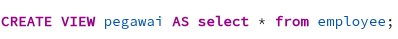
\includegraphics[scale=1.0]{S1.png}

            \end{center}

              Mekanisme sebuah kelas menjadi objek adalah dengan
              mendefinisikan kelas sebagai template yang berisi atribut
              dan metode, kemudian objek dibuat melalui instansiasi kelas,
              yang mengalokasikan memori dan menginisialisasi data sesuai
              konstruktor kelas.

    \end{multicols}

  \item
    \begin{multicols}{2}
            \begin{center}

              \lstinputwithcaption{./code/src/soal2/Main.java}{Main.java}

              \columnbreak

              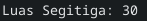
\includegraphics[scale=1.0]{S2.png}

            \end{center}
    \end{multicols}

  \item
    \begin{multicols}{2}
            \begin{center}

              \lstinputwithcaption{./code/src/soal3/Main.java}{Main.java}
              
              \columnbreak


              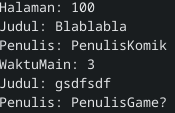
\includegraphics[scale=1.0]{S3.png}

            \end{center}
    \end{multicols}

  \newpage

  \item
          \begin{multicols}{2}
            \begin{center}

              \lstinputwithcaption{./code/src/soal4/Main.java}{Main.java}

              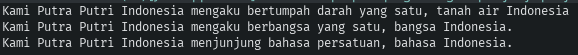
\includegraphics[scale=0.4]{S4.png}

            \end{center}
          \end{multicols}


  \item
          \begin{multicols}{2}
            \begin{center}

              \lstinputwithcaption{./code/src/soal5/Main.java}{Main.java}

              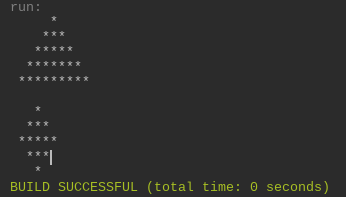
\includegraphics[scale=1.0]{S5.png}

            \end{center}
          \end{multicols}

  \item
          \begin{multicols}{2}
            \begin{center}

              \lstinputwithcaption{./code/src/soal6/Main.java}{Main.java}
              \lstinputwithcaption{./code/src/soal6/Mahasiswa.java}{Mahasiswa.java}
              \columnbreak
              \lstinputwithcaption{./code/src/soal6/Staff.java}{Staff.java}
              \lstinputwithcaption{./code/src/soal6/Dosen.java}{Dosen.java}
              \newpage
              \lstinputwithcaption{./code/src/soal6/Civitas.java}{Civitas.java}

              \columnbreak
              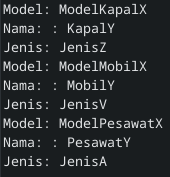
\includegraphics[scale=0.7]{S6.png}

            \end{center}
          \end{multicols}

  \item
          \begin{multicols}{2}
            \begin{center}

              \lstinputwithcaption{./code/src/soal7/Main.java}{Main.java}

              \columnbreak

              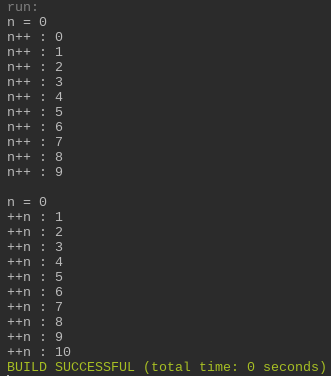
\includegraphics[scale=0.7]{S7.png}

            \end{center}
          \end{multicols}


\end{enumerate}

\end{document}
